\documentclass[a4paper,14pt]{extreport}
  \usepackage[left=1.5cm,right=1.5cm,
      top=1.5cm,bottom=2cm,bindingoffset=0cm]{geometry}
  \usepackage{scrextend}
  \usepackage[T1,T2A]{fontenc}
  \usepackage[utf8]{inputenc}
  \usepackage[english,russian,ukrainian]{babel}
  \usepackage{tabularx}
  \linespread{1.3}
  \usepackage{amssymb}
  \usepackage{color}
  \usepackage{amsmath}
  \usepackage{mathrsfs}
  \usepackage{listings}
  \usepackage{graphicx}
  \graphicspath{ {./images/} }
  \usepackage{lipsum}
  \usepackage{xcolor}
  \usepackage{hyperref}
  \usepackage{tcolorbox}
  \usepackage{tikz}
  \usepackage[framemethod=TikZ]{mdframed}
  \usepackage{wrapfig,boxedminipage,lipsum}
  \mdfdefinestyle{MyFrame}{%
  linecolor=blue,outerlinewidth=2pt,roundcorner=20pt,innertopmargin=\baselineskip,innerbottommargin=\baselineskip,innerrightmargin=20pt,innerleftmargin=20pt,backgroundcolor=gray!50!white}
   \usepackage{csvsimple}
   \usepackage{supertabular}
  \usepackage{pdflscape}
  \usepackage{fancyvrb}
  %\usepackage{comment}
  \usepackage{array,tabularx}
  \usepackage{colortbl}

  \usepackage{varwidth}
  \tcbuselibrary{skins}
  \usepackage{fancybox}
  \usepackage{spreadtab}


  \usepackage{tikz}
  \usepackage[framemethod=TikZ]{mdframed}
  \usepackage{xcolor}
  \usetikzlibrary{calc}
  \makeatletter
  \newlength{\mylength}
  \xdef\CircleFactor{1.1}
  \setlength\mylength{\dimexpr\f@size pt}
  \newsavebox{\mybox}
  \newcommand*\circled[2][draw=blue]{\savebox\mybox{\vbox{\vphantom{WL1/}#1}}\setlength\mylength{\dimexpr\CircleFactor\dimexpr\ht\mybox+\dp\mybox\relax\relax}\tikzset{mystyle/.style={circle,#1,minimum height={\mylength}}}
  \tikz[baseline=(char.base)]
  \node[mystyle] (char) {#2};}
  \makeatother
   % Цвета для гиперссылок
  \definecolor{linkcolor}{rgb}{0, 0.72, 0.92} % цвет ссылок
  \definecolor{urlcolor}{rgb}{0.0, 0.0, 1.0}% цвет гиперссылок
  \hypersetup{pdfstartview=FitH,  linkcolor=linkcolor,urlcolor=urlcolor,citecolor=red, colorlinks=true}

  \definecolor{ggreen}{rgb}{0.4,1,0}
  \definecolor{rred}{rgb}{1,0.1,0.1}
  \definecolor{amber}{rgb}{1.0, 0.75, 0.0}
  \definecolor{babyblue}{rgb}{0.54, 0.81, 0.94}
  \definecolor{amethyst}{rgb}{0.6, 0.4, 0.8}

  \usepackage{float}
  \usepackage{wrapfig}
  \usepackage{framed}
  %for nice Code{
  \lstdefinestyle{customc}{
    belowcaptionskip=1\baselineskip,
    breaklines=true,
    frame=L,
    xleftmargin=\parindent,
    language=C,
    showstringspaces=false,
    basicstyle=\small\ttfamily,
    keywordstyle=\bfseries\color{green!40!black},
    commentstyle=\itshape\color{purple!40!black},
    identifierstyle=\color{blue},
    stringstyle=\color{orange},
  }
  \lstset{escapechar=@,style=customc}
%}

\newcommand{\cam}[1]{\begin{comment}#1\end{comment}}

\begin{document}
%------------------------------1
  \noindent{\color{blue} \rule{\linewidth}{0.7mm}}
  \begin{center}1\end{center}
  \noindent{\color{blue} \rule{\linewidth}{0.7mm}}

\begin{comment}
Перший апарат магнітного запису винайшов і побудував датський інженер Вальдемар Поульсен. Апарат назвали телеграфоном і призначався він для зберігання звуку. Телеграфон був запатентований в 1898 році, і цю дату вважають роком народження магнітного запису.\par
\end{comment}
The first magnetic recording device was invented and built by the Danish engineer Waldemar Poulsen. The device was called a telegraph and was intended for audio storage. The telegraph was patented in 1898, and this date is considered the year of birth of the magnetic record. \par

  \begin{figure}[h]
  \center{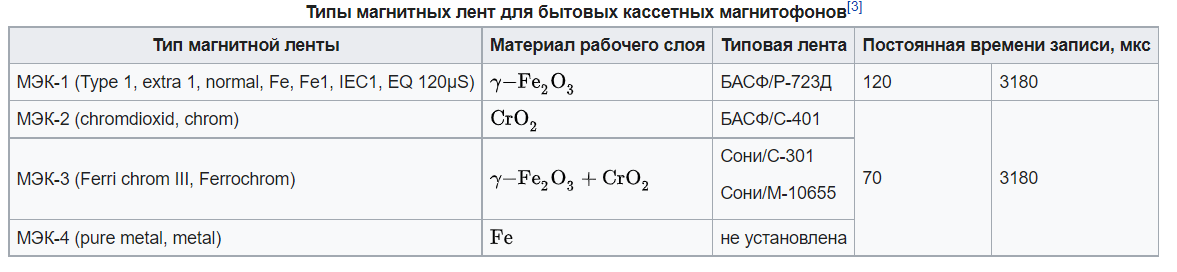
\includegraphics[width=0.9\linewidth]{forp1.png}}
  \end{figure}
Poulsen created several types of magnetic recording devices. In one of them, the wire (recording medium) is wound on a non-magnetic roller, which forms a magnetic working layer on it in the form of a cylindrical spiral. In the process of recording or playing the roller together with the wire
  rotated relative to the magnetic head, which moved parallel to its axis, sliding along the turns of the wire, like a screw thread. An electromagnet was used as the magnetic head, consisting of a rod core, which slid at one end on the carrier, and a coil of copper wire. The head with the core created a fairly strong and concentrated magnetic field, with which you could record sound frequencies. \par
  \begin{comment}
  Поульсен створив кілька різновидів апаратів для магнітного запису. В одному з них дріт (носій запису) намотаний на немагнітний валик, який утворює на ньому магнітний робочий шар у вигляді циліндричної спіралі. В процесі запису або відтворення валик разом з дротом
  обертався відносно магнітної головки, яка переміщалася паралельно його осі, ковзаючи по виткам дроту, як по різьбі гвинта. В ролі магнітної головки використовувався електромагніт, що складався з стрижневого осердя, який одним кінцем ковзав по носію, і котушки мідного дроту. Головка з сердечником створювала досить сильне і сконцентроване магнітне поле, за допомогою якого можна було записувати звукові частоти.\par\end{comment}
%------------------------------2
\noindent{\color{blue} \rule{\linewidth}{0.7mm}}
\begin{center}2\end{center}
\noindent{\color{blue} \rule{\linewidth}{0.7mm}}
and on this slide we can see the structure of the magnetic tape, that is, what it consists of,
%------------------------------3
  \noindent{\color{blue} \rule{\linewidth}{0.7mm}}
  \begin{center}3\end{center}
  \noindent{\color{blue} \rule{\linewidth}{0.7mm}}
 \begin{comment}Основа магнітної стрічки виготовляється з синтетичних матеріалів, найчастіше ацетатцелюлозних (діацетату і триацетату), поліетилентерефталату (лавсану) і полиимидов.\\ % Застосовувалися й інші матеріали (папір, целулоїд, поліетилен, поліхлорвініл), але вони вийшли з ужитку, так як гірше відповідали вимогам, що пред'являються до магнітних стрічок.\\
  В якості робочого шару використовуються порошки оксидів заліза, хрому, кобальту і їх суміші, а також порошки чистих металів. Від складу, товщини і однорідності робочого шару, розмірів і форми частинок магнітного порошку в чому залежать основні характеристики стрічки.\end{comment}

  The basis of the magnetic tape is made of synthetic materials, most often cellulose acetate (diacetate and triacetate), polyethylene terephthalate (mylar) and polyimides. \\% Other materials were used (paper, celluloid, polyethylene, PVC) requirements for magnetic tapes. \\

  Powders of oxides of iron, chromium, cobalt and their mixtures, as well as powders of pure metals are used as a working layer. The main characteristics of the tape depend on the composition, thickness and homogeneity of the working layer, the size and shape of the magnetic powder particles.

%------------------------------4
  \noindent{\color{blue} \rule{\linewidth}{0.7mm}}
  \begin{center}4\end{center}
  \noindent{\color{blue} \rule{\linewidth}{0.7mm}}
 \begin{comment}Фізично технологія запису на жорсткі диски і плівки одна і та ж: дані записуються на намагнічену поверхню вузькими доріжками, на яких відбувається перемикання полярності. Інформація записується послідовністю бітів.\\
  За останнє десятиліття плівка розвивалася не менш, ніж жорсткі диски або транзистори. Перша плівка для зберігання інформації в цифровому вигляді - модель 726 виробництва IBM - могла зберігати 1,1 МБ на котушці. Сьогодні 1 котушка здатна зберігати 15 терабайт даних, а одне роботизоване плівкове сховище - 278 петабайт.\\ 

  Щоб домогтися такого прогресу, інженери пристосували головки для читання і запису рухатися по вкрай вузьких доріжках на плівці - близько 100 нанометрів шириною. Крім цього, довелося зробити зчитувальні головки вужчими - близько 50 нанометрів шириною. При зчитуванні рівень сигналу до шуму теж зменшився, тому довелося маніпулювати розміром і положенням намагнічених гранул і гладкістю поверхні плівки, а також удосконалити процес обробки сигналу і помилок зчитування.\par\end{comment}

Physically, the technology of recording on hard disks and films is the same: the data is recorded on a magnetized surface by narrow tracks on which the polarity is switched. The information is written in a sequence of bits. \\
  Over the last decade, film has evolved no less than hard drives or transistors. The first digital storage film, the IBM Model 726, could hold 1.1 MB on a reel. Today, 1 coil can store 15 terabytes of data, and one robotic film storage - 278 petabytes. \\

  To make this progress, engineers have adapted the read and write heads to move along extremely narrow paths on film - about 100 nanometers wide. In addition, we had to make the reading heads narrower - about 50 nanometers wide. When reading the signal level to noise also decreased, so we had to manipulate the size and position of the magnetized granules and the smoothness of the film surface, as well as improve the process of signal processing and reading errors. \par
%------------------------------5
  \noindent{\color{blue} \rule{\linewidth}{0.7mm}}
  \begin{center}5\end{center}
  \noindent{\color{blue} \rule{\linewidth}{0.7mm}}
 \begin{comment}Як вже було описано раніше, магнітний запис інформації заснована на тому, що багато матеріалів в магнітному полі намагнічуються вздовж його ліній і зберігають цю намагніченість навіть після відключення поля. У магнітних носіях, таких як дискети і HDD, роль бітів виконує намагніченість невеликих ділянок диска. Зі зменшенням розмірів цих ділянок значно зростає обсяг інформації, яку можна записати на пристрої того ж розміру. Зараз один домен комерційно доступних жорстких дисків налічує в собі близько мільйона атомів (кілька нанометрів в діаметрі). Експерименти показують, що розмір комірки можна зменшити до 3-12 атомів.\par
 
   Автори нової роботи домоглися стабільного запису і зберігання інформації протягом декількох годин в одиночних атомах гольмію. Вибір металу вчені пояснюють наступним чином. Будь-яка орбіталь атома може нести на собі жодного, один або два електрони. Магнітні властивості атомів визначаються в основному неспареними електронами, які знаходяться на своїй орбіталі на самоті. Гольмій володіє великою кількістю неспарених електронів і, до того ж, є має найбільший магнітний момент серед елементів періодичної таблиці. Крім того, неспарені електрони атома знаходяться близько до ядра, що забезпечує їх деяку ізольованість від зовнішнього середовища. Тому магнітний стан гольмію може зберігатися досить довгий час.\par
 
   На поверхні оксиду магнію Гольмій відчуває магнітну анізотропію - вона призводить до того, що у атома є два стійких магнітних стана, що визначаються орієнтацією його сумарного спіна. Щоб перейти з одного стану в інший атом повинен подолати енергетичний бар'єр. Чим нижче температура середовища, тим менш імовірний цей перехід. Відповідно цим двох стійким станам і приписуються значення «нуля» і «одиниці».\par\end{comment}

   As previously described, magnetic recording information is based on the fact that many materials in a magnetic field are magnetized along its lines and retain this magnetization even after the field is turned off. In magnetic media, such as floppy disks and HDDs, the role of bits is performed by the magnetization of small areas of the disk. As the size of these areas decreases, the amount of information that can be recorded on devices of the same size increases significantly. Today, one domain of commercially available hard drives has about a million atoms (several nanometers in diameter). Experiments show that cell size can be reduced to 3-12 atoms. \par

  The authors of the new work have achieved stable recording and storage of information for several hours in single holmium atoms. Scientists explain the choice of metal as follows. Any orbital of an atom can carry one, one or two electrons. The magnetic properties of atoms are determined mainly by unpaired electrons, which are in their orbit in solitude. Holmium has a large number of unpaired electrons and, moreover, has the highest magnetic moment among the elements of the periodic table. In addition, the unpaired electrons of the atom are close to the nucleus, which provides some isolation from the environment. Therefore, the magnetic state of holmium can be maintained for a long time. \par

  On the surface of magnesium oxide Holmium undergoes magnetic anisotropy - it leads to the fact that the atom has two stable magnetic states, determined by the orientation of its total spin. To move from one state to another atom must overcome the energy barrier. The lower the ambient temperature, the less likely this transition is. According to these two stable states, the values of "zero" and "one" are attributed. \par

%------------------------------6
\begin{comment}В експерименті вчені створили комірку пам'яті, що складалася з двох атомів гольмію, що знаходяться на поверхні оксиду магнію, який був охолоджений до 1,2 Кельвіна. Для запису і читання вчені використовували скануючий тунельний мікроскоп, який досліджує поверхні за допомогою надзвичайно гострої голки. Операція запису полягала в додаванні до атому певної електричної напруги. Для читання автори використовували ефект тунельного магнітоопору - електричний опір між поверхнею і голкою залежить від напрямків намагніченості кінчика голки і атома гольмію. \par\end{comment}

 In the experiment, scientists created a memory cell consisting of two holmium atoms on the surface of magnesium oxide, which was cooled to 1.2 Kelvin. To write and read, the scientists used a scanning tunneling microscope, which examines surfaces with an extremely sharp needle. The operation of recording was to add to the atom a certain voltage. For reading, the authors used the effect of tunneling magnetoresistance - the electrical resistance between the surface and the needle depends on the directions of magnetization of the tip of the needle and the holmium atom.

%------------------------------7
....

%------------------------------8


$\acute\nu \lambda\varepsilon\tau\rho o \upsilon$










































\end{document}